\documentclass[11pt,a4paper]{article}

\usepackage[margin=1.5cm]{geometry}
\usepackage{amsmath,amssymb}
\usepackage[version=4]{mhchem}
\usepackage{chemfig}
\usepackage{tikz}
\usepackage{booktabs}
\usepackage{longtable}
\usepackage{array}
\usepackage{xcolor}
\usepackage{hyperref}
\usepackage{enumitem}
\usepackage{microtype}

\usetikzlibrary{
  arrows.meta,
  positioning,
  calc,
  decorations.pathmorphing,
  fit
}

\hypersetup{
  colorlinks=true,
  linkcolor=blue!60!black,
  urlcolor=blue!60!black,
  pdftitle={Detailed Glycolysis Reference},
  pdfauthor={Biochemistry Notes}
}

\setlength{\parindent}{0pt}
\setlength{\parskip}{5pt}
\setlength{\tabcolsep}{5pt}
\renewcommand{\arraystretch}{1.2}

\setchemfig{
  atom sep=2.0em,
  bond style={line width=0.8pt},
  double bond sep=2pt
}

\definecolor{invest}{RGB}{205,90,50}
\definecolor{payoff}{RGB}{30,120,90}
\definecolor{transfer}{RGB}{50,95,175}
\definecolor{carbon}{RGB}{45,45,45}

\newcommand{\stepref}[1]{\hyperref[step:#1]{Step~#1}}
\newcommand{\phos}{\mathrm{P_i}}
\newcommand{\ATP}{\ce{ATP}}
\newcommand{\ADP}{\ce{ADP}}
\newcommand{\NAD}{\ce{NAD+}}
\newcommand{\NADH}{\ce{NADH}}
\newcommand{\Enz}[1]{\textbf{Enzyme:} #1}
\newcommand{\Carbon}[1]{\textcolor{carbon}{\mathbf{C}_{#1}}}
\newcommand{\PiGroup}{\ensuremath{\mathrm{-O-PO_3^{2-}}}}
\newcommand{\Note}[1]{\par\smallskip
  \noindent\colorbox{gray!12}{
    \parbox{0.96\linewidth}{#1}
  }\par\smallskip}

\title{\textbf{Glycolysis: Complete Step-by-Step Biochemical Reference}\\
\large Enzymes, Reaction Equations, Carbon Skeletons, Phosphate Transfers,
and Electron Movement}
\author{}
\date{}

\begin{document}

\maketitle

\tableofcontents
\newpage

% =========================================================
\section{Overview of the Glycolytic Pathway}
\label{sec:overview}
% =========================================================

Glycolysis is a ten-reaction metabolic pathway that converts one
six-carbon glucose molecule into two three-carbon pyruvate molecules.

All ten reactions occur in the cytosol.

The pathway is divided into two phases:

\begin{enumerate}[label=\textbf{Phase \arabic*.}]
  \item \textbf{Energy-investment phase: Steps 1--5.}

  Two ATP molecules are consumed. The six-carbon sugar is phosphorylated,
  rearranged, and cleaved into two three-carbon molecules.

  \item \textbf{Energy-payoff phase: Steps 6--10.}

  Two glyceraldehyde-3-phosphate molecules are oxidized and converted
  into pyruvate. Four ATP and two NADH molecules are produced.
\end{enumerate}

\subsection{Whole-pathway diagram}

\begin{figure}[htbp]
\centering
\resizebox{0.96\linewidth}{!}{
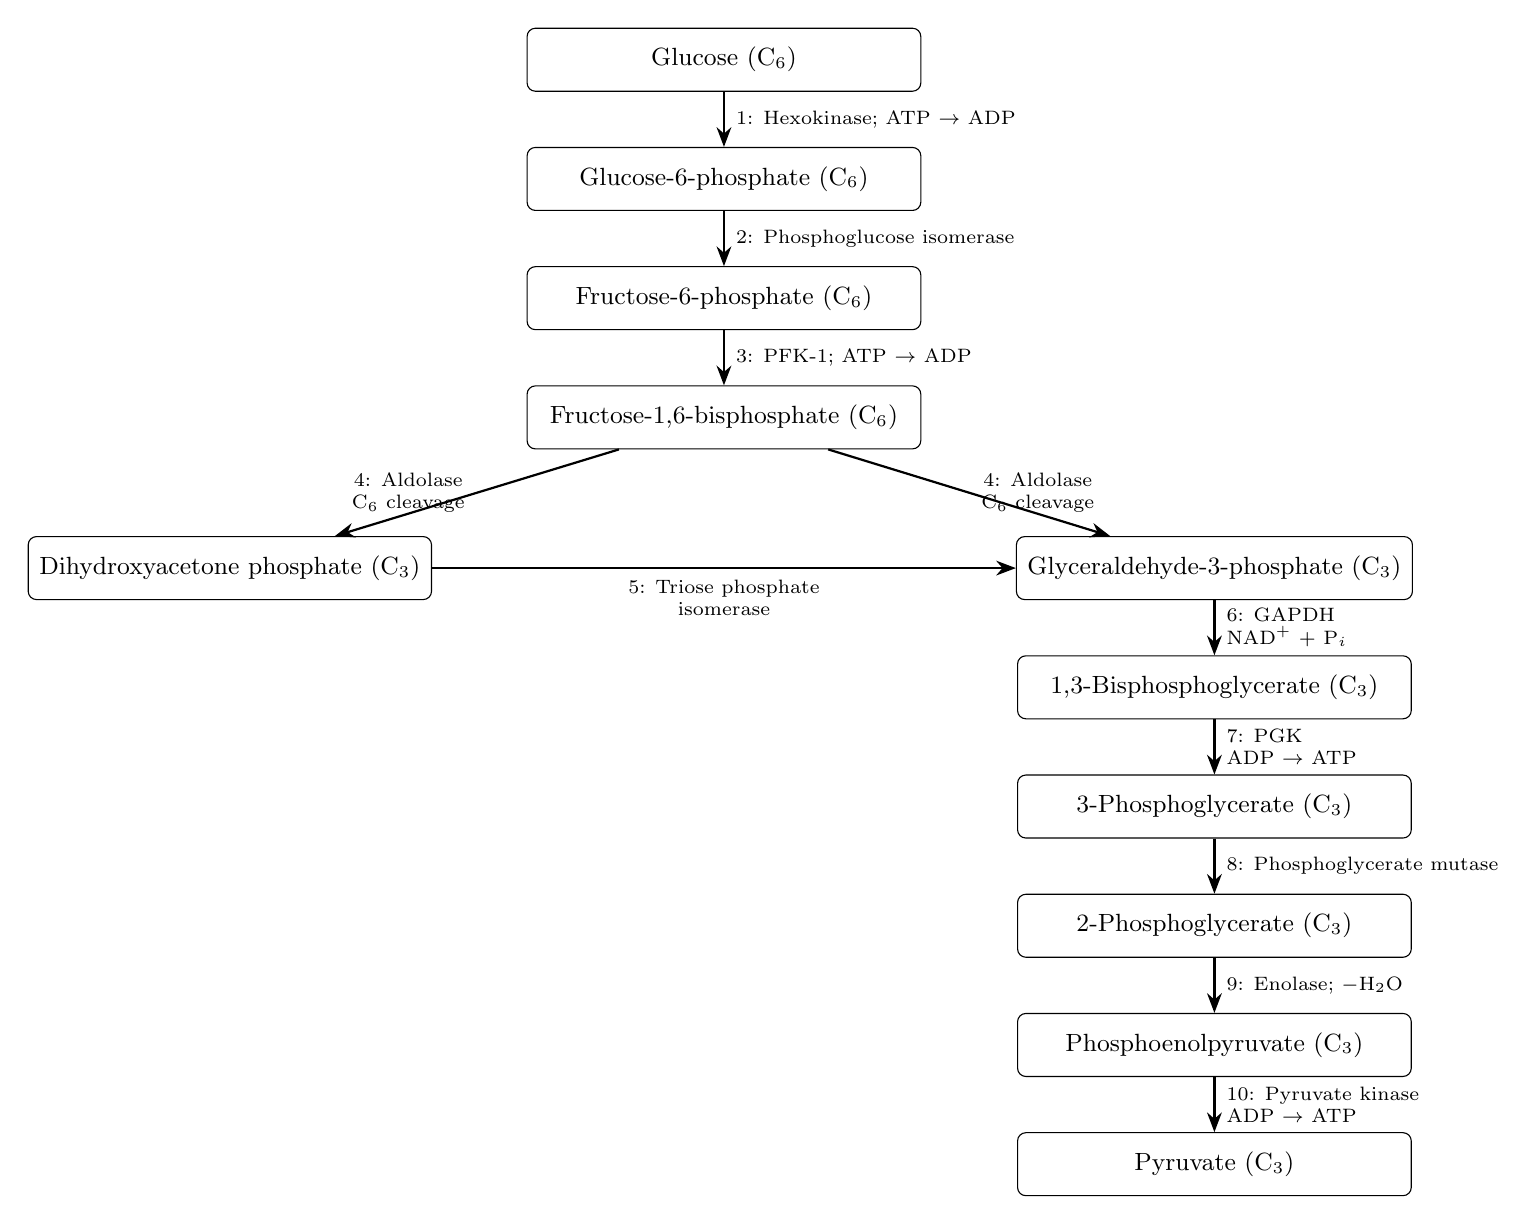
\begin{tikzpicture}[
  node distance=7mm,
  metabolite/.style={
    draw,
    rounded corners=3pt,
    minimum width=5.0cm,
    minimum height=8mm,
    align=center,
    font=\small
  },
  reaction/.style={
    -{Stealth[length=2.5mm]},
    thick
  },
  every node/.style={inner sep=4pt}
]

\node[metabolite] (g) {Glucose (C$_6$)};

\node[metabolite, below=of g] (g6p) {Glucose-6-phosphate (C$_6$)};
\node[metabolite, below=of g6p] (f6p) {Fructose-6-phosphate (C$_6$)};
\node[metabolite, below=of f6p] (fbp) {Fructose-1,6-bisphosphate (C$_6$)};

\node[metabolite, below left=11mm and 12mm of fbp] (dhap)
  {Dihydroxyacetone phosphate (C$_3$)};

\node[metabolite, below right=11mm and 12mm of fbp] (gap)
  {Glyceraldehyde-3-phosphate (C$_3$)};

\node[metabolite, below=of gap] (bpg)
  {1,3-Bisphosphoglycerate (C$_3$)};

\node[metabolite, below=of bpg] (pg3)
  {3-Phosphoglycerate (C$_3$)};

\node[metabolite, below=of pg3] (pg2)
  {2-Phosphoglycerate (C$_3$)};

\node[metabolite, below=of pg2] (pep)
  {Phosphoenolpyruvate (C$_3$)};

\node[metabolite, below=of pep] (pyr)
  {Pyruvate (C$_3$)};

\draw[reaction] (g) -- node[right,font=\scriptsize]
  {1: Hexokinase; ATP $\to$ ADP} (g6p);

\draw[reaction] (g6p) -- node[right,font=\scriptsize]
  {2: Phosphoglucose isomerase} (f6p);

\draw[reaction] (f6p) -- node[right,font=\scriptsize]
  {3: PFK-1; ATP $\to$ ADP} (fbp);

\draw[reaction] (fbp) -- node[left,font=\scriptsize,align=center]
  {4: Aldolase\\C$_6$ cleavage} (dhap);

\draw[reaction] (fbp) -- node[right,font=\scriptsize,align=center]
  {4: Aldolase\\C$_6$ cleavage} (gap);

\draw[reaction] (dhap) -- node[below,font=\scriptsize,align=center]
  {5: Triose phosphate\\isomerase} (gap);

\draw[reaction] (gap) -- node[right,font=\scriptsize,align=left]
  {6: GAPDH\\NAD$^+$ + P$_i$} (bpg);

\draw[reaction] (bpg) -- node[right,font=\scriptsize,align=left]
  {7: PGK\\ADP $\to$ ATP} (pg3);

\draw[reaction] (pg3) -- node[right,font=\scriptsize,align=left]
  {8: Phosphoglycerate mutase} (pg2);

\draw[reaction] (pg2) -- node[right,font=\scriptsize,align=left]
  {9: Enolase; $-\ce{H2O}$} (pep);

\draw[reaction] (pep) -- node[right,font=\scriptsize,align=left]
  {10: Pyruvate kinase\\ADP $\to$ ATP} (pyr);

\end{tikzpicture}
}
\caption{The ten reactions of glycolysis. After step 5, two glyceraldehyde-3-phosphate
molecules proceed through each of steps 6--10.}
\label{fig:overview}
\end{figure}

\Note{
\textbf{Important stoichiometric convention:}
Steps 1--5 occur once per original glucose molecule.
Steps 6--10 occur twice per glucose molecule because two
glyceraldehyde-3-phosphate molecules are formed.
}

% =========================================================
\section{Structural Notation and Atom Tracking}
\label{sec:notation}
% =========================================================

\subsection{Abbreviations}

\begin{longtable}{>{\raggedright\arraybackslash}p{0.20\linewidth}
                  >{\raggedright\arraybackslash}p{0.72\linewidth}}
\toprule
\textbf{Notation} & \textbf{Meaning}\\
\midrule
G6P & Glucose-6-phosphate\\
F6P & Fructose-6-phosphate\\
FBP & Fructose-1,6-bisphosphate\\
DHAP & Dihydroxyacetone phosphate\\
GAP or G3P & Glyceraldehyde-3-phosphate\\
1,3-BPG & 1,3-Bisphosphoglycerate\\
3-PG & 3-Phosphoglycerate\\
2-PG & 2-Phosphoglycerate\\
PEP & Phosphoenolpyruvate\\
P$_i$ & Inorganic phosphate\\
ATP & Adenosine triphosphate\\
ADP & Adenosine diphosphate\\
NAD$^+$ & Oxidized electron acceptor\\
NADH & Reduced electron carrier\\
PFK-1 & Phosphofructokinase-1\\
GAPDH & Glyceraldehyde-3-phosphate dehydrogenase\\
PGK & Phosphoglycerate kinase\\
\bottomrule
\end{longtable}

\subsection{Carbon numbering}

Carbon atoms are numbered according to their positions in the
intermediates, not according to a universal numbering system maintained
unchanged through every reaction.

\begin{itemize}
  \item Glucose contains six carbon atoms, numbered C1--C6.
  \item The isomerization in step 2 converts an aldose into a ketose.
  \item Aldolase cleaves the six-carbon intermediate between C3 and C4.
  \item The resulting triose phosphates each contain three carbon atoms.
  \item From step 6 onward, each triose molecule follows the same
  five-reaction sequence.
\end{itemize}

The original glucose carbon atoms are conserved: glycolysis does not
release carbon dioxide.

\subsection{Phosphate notation}

In structural formulas, the phosphate ester group is abbreviated as
\[
\mathrm{-O-PO_3^{2-}}.
\]

This notation shows the essential connectivity between the sugar oxygen
and phosphorus. It suppresses some protonation details because the
actual charge distribution depends on pH and the ionic environment.

The phosphate group donated by ATP is transferred to the sugar through
an oxygen atom. It is not transferred as an isolated phosphorus atom.

% =========================================================
\section{Step 1: Phosphorylation of Glucose}
\label{step:1}
% =========================================================

\subsection{Reaction}

\[
\boxed{
\ce{Glucose + ATP ->[Hexokinase][Mg^{2+}] Glucose-6-phosphate + ADP}
}
\]

\Enz{Hexokinase. In liver and pancreatic beta cells, glucokinase
(hexokinase IV) performs the corresponding reaction.}

\subsection{Reactants and products}

\begin{itemize}
  \item Reactants: glucose, ATP.
  \item Products: glucose-6-phosphate, ADP.
  \item Cofactor: usually Mg$^{2+}$, which helps coordinate nucleotide
  phosphate groups.
  \item ATP consumed: one molecule per glucose.
\end{itemize}

\subsection{Structural representation}

\[
\ce{HOCH2-(CHOH)4-CHO}
\quad \text{(open-chain glucose, schematic)}
\]

\[
\ce{Glucose + ATP -> Glucose-6-phosphate + ADP}
\]

In the open-chain representation, the terminal C6 hydroxyl group
becomes a phosphate ester:

\[
\ce{-CH2OH -> -CH2OPO3^{2-}}.
\]

\subsection{Bond and atom changes}

\begin{enumerate}
  \item The C6 hydroxyl oxygen of glucose acts as the acceptor atom
  for the phosphoryl group.
  \item The terminal phosphate of ATP is transferred to this oxygen.
  \item The C6 oxygen forms a bond to phosphorus.
  \item ATP becomes ADP after losing its terminal phosphoryl group.
  \item The six-carbon skeleton of glucose remains intact.
\end{enumerate}

\subsection{Electron movement}

The hydroxyl oxygen is the nucleophile in the phosphoryl-transfer
reaction. It attacks the terminal phosphorus of ATP, while the
phosphoryl-transfer transition state is stabilized by the enzyme
and Mg$^{2+}$.

This is a nucleophilic substitution at phosphorus, not oxidation of
the glucose carbon skeleton.

\subsection{Energy and physiological significance}

One ATP is consumed. The resulting glucose-6-phosphate is charged
and does not readily cross the plasma membrane through glucose
transporters. Phosphorylation also prepares glucose for subsequent
metabolic reactions.

\Note{
\textbf{Reference:} \stepref{1}. The phosphate is attached to C6,
not C1. No NADH is produced.
}

% =========================================================
\section{Step 2: Isomerization of Glucose-6-phosphate}
\label{step:2}
% =========================================================

\subsection{Reaction}

\[
\boxed{
\ce{Glucose-6-phosphate <=>[Phosphoglucose\ isomerase]
Fructose-6-phosphate}
}
\]

\Enz{Phosphoglucose isomerase, also called glucose-6-phosphate
isomerase.}

\subsection{Reactants and products}

\begin{itemize}
  \item Reactant: glucose-6-phosphate.
  \item Product: fructose-6-phosphate.
  \item ATP consumed: none.
  \item NAD$^+$ consumed: none.
\end{itemize}

\subsection{Functional-group change}

Glucose-6-phosphate is an aldose phosphate in its open-chain form.
Fructose-6-phosphate is a ketose phosphate.

The net rearrangement moves the carbonyl functionality from C1
to C2 without changing the six-carbon skeleton or the position
of the phosphate group.

\[
\ce{
CHO-(CHOH)4-CH2OPO3^{2-}
<=>
CH2OH-CO-(CHOH)3-CH2OPO3^{2-}
}
\]

This expression is a schematic connectivity comparison; the exact
stereochemistry and hydroxyl positions are omitted.

\subsection{Mechanistic sequence}

\begin{enumerate}
  \item The cyclic sugar opens to the linear form.
  \item A catalytic base removes a proton adjacent to the carbonyl
  while the enzyme stabilizes the developing intermediate.
  \item An enediol or enediolate-like intermediate is formed.
  \item Proton transfer and carbonyl reformation produce the ketose.
  \item The product can cyclize again.
\end{enumerate}

\subsection{Electron movement}

The transformation is an intramolecular redox-neutral rearrangement.
Electrons are redistributed within the sugar during the enediol-mediated
isomerization.

There is no net transfer of electrons to NAD$^+$, and there is no net
oxidation or reduction of the overall sugar molecule.

\subsection{Why this step matters}

Moving the carbonyl from C1 to C2 makes the later cleavage of
fructose-1,6-bisphosphate possible in a way that produces two
three-carbon phosphate intermediates.

\Note{
\textbf{Reference:} \stepref{2}. This is an isomerization, not a
phosphorylation or oxidation reaction.
}

% =========================================================
\section{Step 3: Phosphorylation of Fructose-6-phosphate}
\label{step:3}
% =========================================================

\subsection{Reaction}

\[
\boxed{
\ce{
Fructose-6-phosphate + ATP
->[Phosphofructokinase-1][Mg^{2+}]
Fructose-1,6-bisphosphate + ADP
}
}
\]

\Enz{Phosphofructokinase-1 (PFK-1).}

\subsection{Reactants and products}

\begin{itemize}
  \item Reactants: fructose-6-phosphate, ATP.
  \item Products: fructose-1,6-bisphosphate, ADP.
  \item ATP consumed: one molecule per glucose.
  \item Cofactor: Mg$^{2+}$.
\end{itemize}

\subsection{Structural change}

A phosphate group is added to the C1 hydroxyl group of
fructose-6-phosphate.

The existing phosphate remains at C6.

\[
\ce{
F6P + ATP -> F1,6BP + ADP
}
\]

The product has two separate phosphate ester groups, one at C1
and one at C6. The prefix \emph{bisphosphate} indicates that
the two phosphate groups are attached at distinct positions.

\subsection{Electron movement}

The C1 hydroxyl oxygen attacks the terminal phosphorus of ATP.
The enzyme facilitates transfer of the phosphoryl group, and ATP
becomes ADP.

As in step 1, this is a phosphoryl-transfer reaction rather than
an oxidation-reduction reaction.

\subsection{Energy and regulation}

This reaction consumes the second ATP molecule of glycolysis.

PFK-1 is a major regulatory enzyme. Its activity responds to the
cell's energy state and other metabolic signals. The forward reaction
is strongly favorable under typical cellular conditions.

\Note{
\textbf{Reference:} \stepref{3}. At the end of this step, two ATP
molecules have been invested per original glucose.
}

% =========================================================
\section{Step 4: Cleavage of Fructose-1,6-bisphosphate}
\label{step:4}
% =========================================================

\subsection{Reaction}

\[
\boxed{
\ce{
Fructose-1,6-bisphosphate
<=>[Aldolase]
Glyceraldehyde-3-phosphate + Dihydroxyacetone phosphate
}
}
\]

\Enz{Fructose-bisphosphate aldolase.}

\subsection{Reactants and products}

\begin{itemize}
  \item Reactant: fructose-1,6-bisphosphate, containing six carbons.
  \item Products: glyceraldehyde-3-phosphate (GAP) and
  dihydroxyacetone phosphate (DHAP), each containing three carbons.
  \item ATP consumed: none.
  \item NAD$^+$ consumed: none.
\end{itemize}

\subsection{Carbon-skeleton cleavage}

The six-carbon substrate is cleaved between C3 and C4.

\[
\boxed{
\mathrm{C_6 \longrightarrow C_3 + C_3}
}
\]

The products are not chemically identical:

\begin{itemize}
  \item GAP contains an aldehyde group in its open-chain form.
  \item DHAP contains a ketone group in its open-chain form.
\end{itemize}

Both products carry one phosphate group.

\subsection{Mechanistic interpretation}

The enzyme stabilizes the intermediates required for cleavage of
the carbon-carbon bond. In class I aldolases, an active-site lysine
forms a Schiff-base intermediate with the substrate. Class II
aldolases instead use a metal ion to stabilize charged intermediates.

The detailed mechanism depends on the aldolase class.

\subsection{Electron movement}

This reaction redistributes bonding electrons as a carbon-carbon
bond is cleaved. It is not a net oxidation-reduction reaction.

No carbon is lost as carbon dioxide. All six carbon atoms from
glucose remain in the two three-carbon products.

\Note{
\textbf{Reference:} \stepref{4}. One molecule of glucose produces
one GAP and one DHAP.
}

% =========================================================
\section{Step 5: Isomerization of DHAP to GAP}
\label{step:5}
% =========================================================

\subsection{Reaction}

\[
\boxed{
\ce{
Dihydroxyacetone phosphate
<=>[Triose\ phosphate\ isomerase]
Glyceraldehyde-3-phosphate
}
}
\]

\Enz{Triose phosphate isomerase (TPI).}

\subsection{Reactants and products}

\begin{itemize}
  \item Reactant: DHAP.
  \item Product: GAP.
  \item ATP consumed: none.
  \item NAD$^+$ consumed: none.
\end{itemize}

\subsection{Structural transformation}

DHAP and GAP are three-carbon constitutional isomers. The
carbonyl group changes from a ketone at C2 to an aldehyde at C1
in the open-chain representation.

\[
\ce{
HOCH2-CO-CH2OPO3^{2-}
<=> 
OHC-CHOH-CH2OPO3^{2-}
}
\]

The formula above is schematic and suppresses protonation and
stereochemical details.

\subsection{Mechanism}

\begin{enumerate}
  \item An active-site base removes a proton from DHAP.
  \item An enediol or enediolate intermediate is formed.
  \item Proton transfer occurs.
  \item Reformation of the carbonyl produces GAP.
\end{enumerate}

The enzyme prevents undesirable side reactions and accelerates
the reversible interconversion.

\subsection{Electron movement}

The electrons are redistributed within the three-carbon skeleton.
There is no net electron transfer to NAD$^+$ and no net oxidation
of the substrate.

\subsection{Stoichiometric consequence}

The GAP produced in step 4 is retained, and the DHAP is converted
into a second GAP.

Therefore:

\[
\boxed{
1\ \text{glucose} \longrightarrow 2\ \text{GAP}
}
\]

Every subsequent reaction occurs twice per glucose molecule.

\Note{
\textbf{Reference:} \stepref{5}. The pathway now contains two
equivalents of GAP.
}

% =========================================================
\section{Step 6: Oxidation and Phosphorylation of GAP}
\label{step:6}
% =========================================================

\subsection{Reaction}

\[
\boxed{
\ce{
GAP + NAD+ + P_i
<=>[GAPDH]
1,3-BPG + NADH + H+
}
}
\]

\Enz{Glyceraldehyde-3-phosphate dehydrogenase (GAPDH).}

\subsection{Reactants and products}

For each GAP molecule:

\begin{itemize}
  \item Reactants: GAP, NAD$^+$, inorganic phosphate.
  \item Products: 1,3-bisphosphoglycerate, NADH, H$^+$.
  \item ATP consumed: none.
  \item NAD$^+$ reduced: one molecule.
\end{itemize}

Because two GAP molecules are processed per glucose, the net
contribution of this step is:

\[
\ce{
2 GAP + 2 NAD+ + 2 P_i
-> 2 1,3-BPG + 2 NADH + 2 H+
}
\]

\subsection{Structural transformation}

The aldehyde carbon of GAP is oxidized to the acyl-phosphate
carbon of 1,3-BPG.

\[
\ce{
OHC-CHOH-CH2OPO3^{2-}
}
\]

\[
\Downarrow
\]

\[
\ce{
O=C(OPO3^{2-})-CHOH-CH2OPO3^{2-}
}
\]

These are schematic open-chain representations. The first
phosphate in the product is an acyl phosphate; the second is
the pre-existing phosphate ester.

\subsection{Where the phosphate comes from}

The phosphate attached at C3 of GAP is already present before
this reaction. The new phosphate at C1 comes from inorganic
phosphate, P$_i$.

It does \textbf{not} come from ATP.

\subsection{Electron transfer}

This is the principal oxidation-reduction step of glycolysis.

\begin{enumerate}
  \item The aldehyde group of GAP is oxidized.
  \item Electrons are transferred to NAD$^+$ through the enzyme's
  catalytic mechanism.
  \item NAD$^+$ accepts a hydride equivalent, corresponding to
  two electrons and one proton, to form NADH.
  \item An additional proton may be released to solution, depending
  on the chosen reaction convention.
\end{enumerate}

The simplified redox bookkeeping is:

\[
\boxed{
\ce{NAD+ + 2H -> NADH + H+}
}
\]

Here, the notation represents net reducing-equivalent transfer,
not the presence of free atomic hydrogen as a reaction intermediate.

The GAPDH mechanism uses a catalytic cysteine residue to form
a covalent intermediate with the aldehyde-derived substrate.
Oxidation generates a high-energy acyl intermediate, which is
then attacked by inorganic phosphate to form the acyl phosphate
of 1,3-BPG.

\subsection{Energy capture}

The energy released during oxidation is conserved in two forms:

\begin{itemize}
  \item The reduced electron carrier NADH.
  \item The high phosphoryl-transfer potential of 1,3-BPG.
\end{itemize}

This is an example of coupling oxidation to formation of a
high-energy phosphate compound.

\Note{
\textbf{Reference:} \stepref{6}. Per glucose, two NADH molecules
are produced. No ATP is produced directly in this reaction.
}

% =========================================================
\section{Step 7: ATP Production from 1,3-BPG}
\label{step:7}
% =========================================================

\subsection{Reaction}

\[
\boxed{
\ce{
1,3-BPG + ADP
<=>[Phosphoglycerate\ kinase]
3-PG + ATP
}
}
\]

\Enz{Phosphoglycerate kinase (PGK).}

\subsection{Reactants and products}

For each 1,3-BPG molecule:

\begin{itemize}
  \item Reactants: 1,3-BPG, ADP.
  \item Products: 3-phosphoglycerate, ATP.
  \item ATP produced: one molecule.
\end{itemize}

Per glucose:

\[
\ce{
2 1,3-BPG + 2 ADP
-> 2 3-PG + 2 ATP
}
\]

\subsection{Phosphate transfer}

The phosphate attached to C1 of 1,3-BPG is transferred to ADP.

\[
\boxed{
\text{C1 acyl phosphate}
\longrightarrow
\text{ADP}
\longrightarrow
\text{ATP}
}
\]

The phosphate at C3 remains attached to the three-carbon skeleton.
The product is 3-phosphoglycerate.

\subsection{Electron movement}

This is a phosphoryl-transfer reaction, not an oxidation-reduction
reaction.

The reaction does not transfer electrons to NAD$^+$, and the
carbon oxidation state does not undergo a net redox change.

The enzyme facilitates phosphoryl transfer from the high-energy
acyl phosphate to ADP.

\subsection{Energy accounting}

This is the first ATP-producing reaction of glycolysis.

Because two molecules of 1,3-BPG are generated per glucose,
this step produces two ATP molecules per glucose.

The process is called \textbf{substrate-level phosphorylation}:
ATP is formed by direct transfer of a phosphoryl group from a
metabolic intermediate to ADP.

\Note{
\textbf{Reference:} \stepref{7}. Two ATP molecules are generated
per glucose. This compensates for the two ATP molecules consumed
in steps 1 and 3, but does not yet create a net gain.
}

% =========================================================
\section{Step 8: Phosphate Migration}
\label{step:8}
% =========================================================

\subsection{Reaction}

\[
\boxed{
\ce{
3-PG <=>[Phosphoglycerate\ mutase] 2-PG
}
}
\]

\Enz{Phosphoglycerate mutase.}

\subsection{Reactants and products}

\begin{itemize}
  \item Reactant: 3-phosphoglycerate.
  \item Product: 2-phosphoglycerate.
  \item ATP consumed or produced: none.
  \item NAD$^+$ consumed: none.
\end{itemize}

\subsection{Structural transformation}

The phosphate group changes position on the three-carbon skeleton.

\[
\ce{
^-OOC-CH(OH)-CH2OPO3^{2-}
}
\]

\[
\Downarrow
\]

\[
\ce{
^-OOC-CH(OPO3^{2-})-CH2OH
}
\]

The phosphate moves from C3 to C2.

\subsection{Mechanistic sequence}

In the common phosphohistidine-dependent mechanism:

\begin{enumerate}
  \item The enzyme transfers a phosphate group to C2, forming
  a transient bisphosphorylated intermediate.
  \item The original C3 phosphate is removed.
  \item The result is 2-phosphoglycerate, with phosphate attached
  at C2.
\end{enumerate}

Some organisms use mechanistically distinct phosphoglycerate
mutases, but the net transformation is the same.

\subsection{Electron movement}

This is an intramolecular rearrangement mediated by the enzyme.
No net electron transfer to NAD$^+$ occurs.

\subsection{Why the phosphate moves}

Moving the phosphate to C2 prepares the molecule for dehydration
in step 9. The resulting phosphoenolpyruvate has a high phosphoryl-
transfer potential.

\Note{
\textbf{Reference:} \stepref{8}. The phosphate is relocated;
ATP is neither consumed nor generated.
}

% =========================================================
\section{Step 9: Dehydration to Phosphoenolpyruvate}
\label{step:9}
% =========================================================

\subsection{Reaction}

\[
\boxed{
\ce{
2-PG
<=>[Enolase]
PEP + H2O
}
}
\]

\Enz{Enolase.}

\subsection{Reactants and products}

\begin{itemize}
  \item Reactant: 2-phosphoglycerate.
  \item Products: phosphoenolpyruvate (PEP), water.
  \item ATP consumed or produced: none.
  \item NAD$^+$ consumed: none.
\end{itemize}

\subsection{Structural transformation}

The reaction removes the elements of water from 2-phosphoglycerate
and creates a carbon-carbon double bond.

\[
\ce{
^-OOC-CH(OPO3^{2-})-CH2OH
}
\]

\[
\Downarrow\quad -\ce{H2O}
\]

\[
\ce{
^-OOC-C(OPO3^{2-})=CH2
}
\]

The displayed formulas are schematic representations of the
connectivity of the substrate and product.

\subsection{Bond changes}

\begin{enumerate}
  \item A proton is removed from one carbon.
  \item The hydroxyl group is eliminated from the adjacent carbon.
  \item The electrons are redistributed to form the C=C double bond.
  \item Water is released.
  \item The product is the enol phosphate PEP.
\end{enumerate}

\subsection{Electron movement}

The enzyme promotes an elimination reaction. Bond electrons are
redistributed within the carbon skeleton, resulting in the double
bond of PEP.

There is no net transfer of electrons to NAD$^+$ and no direct
ATP formation in this step.

\subsection{Energy significance}

PEP has a high phosphoryl-transfer potential. Its conversion to
pyruvate is strongly favorable because the initial enol product
can tautomerize to the more stable keto form of pyruvate.

\Note{
\textbf{Reference:} \stepref{9}. Dehydration creates the
high-energy enol phosphate used in step 10.
}

% =========================================================
\section{Step 10: ATP Production and Formation of Pyruvate}
\label{step:10}
% =========================================================

\subsection{Reaction}

\[
\boxed{
\ce{
PEP + ADP + H+
->[Pyruvate\ kinase][Mg^{2+},K+]
Pyruvate + ATP
}
}
\]

\Enz{Pyruvate kinase.}

\subsection{Reactants and products}

For each PEP molecule:

\begin{itemize}
  \item Reactants: PEP, ADP.
  \item Products: pyruvate, ATP.
  \item ATP produced: one molecule.
  \item Required ions commonly include Mg$^{2+}$ and K$^+$.
\end{itemize}

Per glucose:

\[
\ce{
2 PEP + 2 ADP + 2H+
-> 2 Pyruvate + 2 ATP
}
\]

The exact proton coefficient depends on the protonation conventions
used for the metabolites.

\subsection{Phosphate transfer}

The phosphate group of PEP is transferred to ADP.

\[
\boxed{
\text{PEP}
\longrightarrow
\text{ADP}
\longrightarrow
\text{ATP}
}
\]

The three-carbon skeleton becomes pyruvate.

\subsection{Electron movement and tautomerization}

The initial product of phosphoryl transfer is an enol form of
pyruvate. It undergoes keto-enol tautomerization to produce the
more stable keto form.

The electron redistribution associated with this tautomerization
helps make the overall reaction strongly favorable.

This is not an additional oxidation of pyruvate. Rather, the
reaction couples phosphoryl transfer with formation of the
thermodynamically favored keto product.

\subsection{Energy accounting}

This is the second ATP-producing reaction of glycolysis.

Two PEP molecules are produced per glucose, so this step generates
two ATP molecules per glucose.

\Note{
\textbf{Reference:} \stepref{10}. The final glycolytic product is
two pyruvate molecules, and this step produces the final two ATP
molecules of the pathway.
}

% =========================================================
\section{Complete Reaction Table}
\label{sec:reaction-table}
% =========================================================

\small

\begin{longtable}{
  >{\centering\arraybackslash}p{0.055\linewidth}
  >{\raggedright\arraybackslash}p{0.245\linewidth}
  >{\raggedright\arraybackslash}p{0.36\linewidth}
  >{\centering\arraybackslash}p{0.105\linewidth}
  >{\centering\arraybackslash}p{0.12\linewidth}
}
\toprule
\textbf{Step} &
\textbf{Enzyme} &
\textbf{Main transformation} &
\textbf{ATP} &
\textbf{Redox}\\
\midrule
\endfirsthead

\toprule
\textbf{Step} &
\textbf{Enzyme} &
\textbf{Main transformation} &
\textbf{ATP} &
\textbf{Redox}\\
\midrule
\endhead

1 & Hexokinase &
Glucose $\to$ glucose-6-phosphate &
$-1$ &
No\\

2 & Phosphoglucose isomerase &
G6P $\to$ F6P &
$0$ &
No\\

3 & Phosphofructokinase-1 &
F6P $\to$ fructose-1,6-bisphosphate &
$-1$ &
No\\

4 & Aldolase &
FBP $\to$ GAP + DHAP &
$0$ &
No\\

5 & Triose phosphate isomerase &
DHAP $\to$ GAP &
$0$ &
No\\

6 & GAP dehydrogenase &
GAP $\to$ 1,3-BPG; NAD$^+$ reduced &
$0$ &
Yes\\

7 & Phosphoglycerate kinase &
1,3-BPG $\to$ 3-PG &
$+2$ per glucose &
No\\

8 & Phosphoglycerate mutase &
3-PG $\to$ 2-PG &
$0$ &
No\\

9 & Enolase &
2-PG $\to$ PEP + water &
$0$ &
No\\

10 & Pyruvate kinase &
PEP $\to$ pyruvate &
$+2$ per glucose &
No\\

\bottomrule
\end{longtable}

\normalsize

\textbf{ATP accounting:}

\[
\begin{aligned}
\text{ATP consumed} &= 2,\\
\text{ATP produced} &= 4,\\
\text{Net ATP} &= 4-2=2.
\end{aligned}
\]

\textbf{NADH accounting:}

\[
\boxed{
1\ \text{glucose} \longrightarrow 2\ \text{NADH}
}
\]

% =========================================================
\section{Phosphate-Transfer Map}
\label{sec:phosphate-map}
% =========================================================

The pathway uses two distinct sources of phosphate.

\subsection{Phosphate groups donated by ATP}

\begin{enumerate}
  \item Step 1: ATP donates a phosphate to glucose at C6.
  \item Step 3: ATP donates a phosphate to fructose-6-phosphate at C1.
\end{enumerate}

These are the two ATP-investment reactions.

\subsection{Phosphate groups donated by inorganic phosphate}

\begin{enumerate}
  \item Step 6: inorganic phosphate is incorporated into 1,3-BPG
  during the oxidation of GAP.
\end{enumerate}

The phosphate incorporated at C1 of 1,3-BPG is not donated by ATP.

\subsection{Phosphate groups transferred to ADP}

\begin{enumerate}
  \item Step 7: 1,3-BPG transfers its C1 phosphate to ADP.
  \item Step 10: PEP transfers its phosphate to ADP.
\end{enumerate}

Both reactions produce ATP by substrate-level phosphorylation.

\subsection{Simplified phosphate-flow diagram}

\begin{figure}[htbp]
\centering
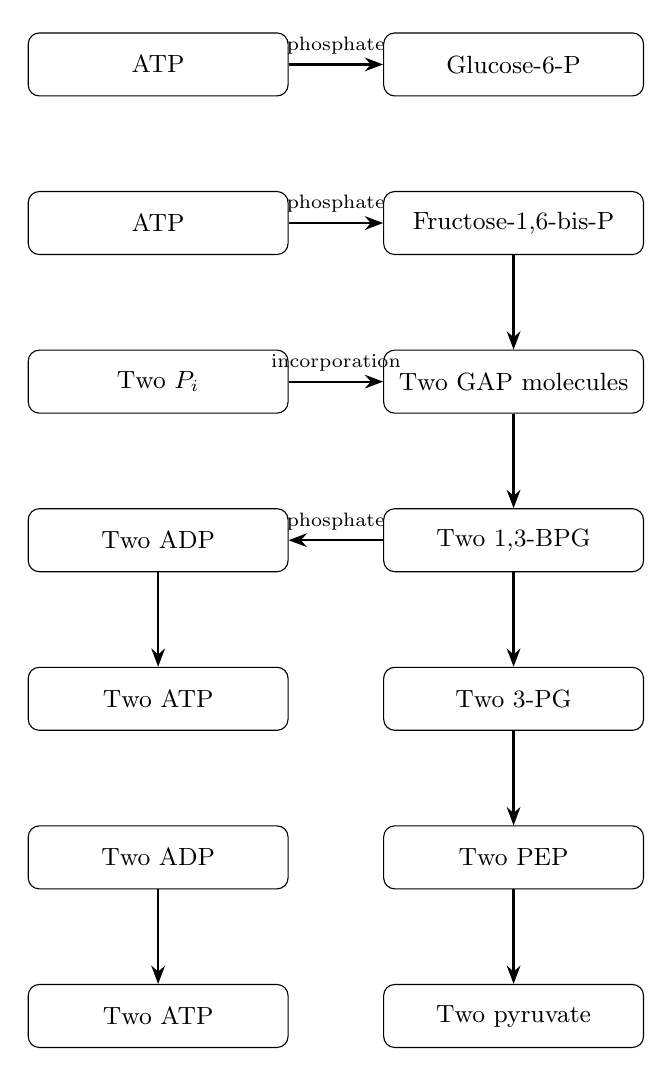
\begin{tikzpicture}[
  box/.style={
    draw,
    rounded corners,
    align=center,
    minimum width=3.3cm,
    minimum height=8mm,
    font=\small
  },
  arr/.style={-{Stealth},thick},
  node distance=12mm
]

\node[box] (atp1) {ATP};
\node[box,right=of atp1] (g6p) {Glucose-6-P};
\node[box,below=of atp1] (atp2) {ATP};
\node[box,right=of atp2] (fbp) {Fructose-1,6-bis-P};

\node[box,below=of fbp] (gap) {Two GAP molecules};
\node[box,left=of gap] (pi) {Two $P_i$};
\node[box,below=of gap] (bpg) {Two 1,3-BPG};
\node[box,left=of bpg] (adp1) {Two ADP};
\node[box,below=of bpg] (pg) {Two 3-PG};
\node[box,left=of pg] (atpout1) {Two ATP};
\node[box,below=of pg] (pep) {Two PEP};
\node[box,left=of pep] (adp2) {Two ADP};
\node[box,below=of pep] (pyr) {Two pyruvate};
\node[box,left=of pyr] (atpout2) {Two ATP};

\draw[arr] (atp1) -- node[above,font=\scriptsize]{phosphate} (g6p);
\draw[arr] (atp2) -- node[above,font=\scriptsize]{phosphate} (fbp);
\draw[arr] (fbp) -- (gap);
\draw[arr] (pi) -- node[above,font=\scriptsize]{incorporation} (gap);
\draw[arr] (gap) -- (bpg);
\draw[arr] (bpg) -- node[above,font=\scriptsize]{phosphate} (adp1);
\draw[arr] (bpg) -- (pg);
\draw[arr] (adp1) -- (atpout1);
\draw[arr] (pg) -- (pep);
\draw[arr] (adp2) -- (atpout2);
\draw[arr] (pep) -- (pyr);

\end{tikzpicture}
\caption{Schematic accounting for phosphate investment and transfer.
The map is an accounting aid rather than a literal spatial model
of enzyme-bound intermediates.}
\label{fig:phosphate-flow}
\end{figure}

% =========================================================
\section{Electron-Transfer Map}
\label{sec:electron-map}
% =========================================================

Only step 6 directly reduces NAD$^+$ during glycolysis.

\[
\boxed{
\ce{2 GAP + 2 NAD+ + 2 P_i
-> 2 1,3-BPG + 2 NADH + 2 H+}
}
\]

The important distinction is between oxidation of the carbon
substrate and phosphoryl transfer:

\begin{itemize}
  \item Step 6 oxidizes GAP and reduces NAD$^+$.
  \item Step 7 transfers a phosphate group to ADP.
  \item Step 10 transfers another phosphate group to ADP.
\end{itemize}

No molecular oxygen is consumed directly in the ten reactions
of glycolysis. Nevertheless, glycolysis contains an oxidation
reaction because NAD$^+$ acts as an electron acceptor.

\subsection{What happens to the NADH?}

NADH must eventually be reoxidized to NAD$^+$ if glycolysis
is to continue.

Under aerobic conditions, the reducing equivalents can be
transferred to mitochondrial oxidative metabolism through
appropriate shuttle systems.

Under anaerobic conditions in animal cells, lactate dehydrogenase
can reduce pyruvate to lactate:

\[
\ce{Pyruvate + NADH + H+ <=> Lactate + NAD+}.
\]

This reaction regenerates NAD$^+$, allowing GAPDH to continue
operating. It is a subsequent reaction, not one of the ten
reactions of glycolysis itself.

% =========================================================
\section{Overall Stoichiometry}
\label{sec:overall}
% =========================================================

The overall glycolytic reaction is conventionally written as

\[
\boxed{
\begin{aligned}
\ce{Glucose}
&+\ce{2 NAD+}
+\ce{2 ADP}
+\ce{2 P_i}\\
&\longrightarrow
\ce{2 Pyruvate}
+\ce{2 NADH}
+\ce{2 H+}
+\ce{2 ATP}
+\ce{2 H2O}.
\end{aligned}
}
\]

This equation uses a common biochemical protonation convention.
The exact coefficient for protons depends on how ionic species
are represented.

\subsection{Net yield per glucose}

\begin{center}
\begin{tabular}{lc}
\toprule
\textbf{Quantity} & \textbf{Net yield}\\
\midrule
Glucose consumed & 1\\
Pyruvate produced & 2\\
ATP consumed & 2\\
ATP produced & 4\\
ATP net gain & 2\\
NADH produced & 2\\
Carbon dioxide produced directly & 0\\
\bottomrule
\end{tabular}
\end{center}

\subsection{Carbon balance}

\[
\boxed{
\ce{C6H12O6 -> 2 C3\text{-}carbon\ products}
}
\]

The notation above emphasizes carbon accounting rather than
serving as a complete balanced chemical equation.

The six glucose carbon atoms remain in the two pyruvate molecules.
No carbon is lost as carbon dioxide during glycolysis.

% =========================================================
\section{Key Biochemical Conclusions}
\label{sec:conclusions}
% =========================================================

\begin{enumerate}
  \item Glycolysis consists of ten enzyme-catalyzed reactions.

  \item The first five reactions consume two ATP molecules and
  generate two GAP molecules.

  \item The last five reactions occur twice per original glucose.

  \item GAP is oxidized in step 6, generating two NADH molecules
  per glucose.

  \item Phosphate transfer to ADP occurs in steps 7 and 10,
  generating four ATP molecules in total.

  \item The net ATP gain is two ATP molecules per glucose.

  \item Steps 1, 3, and 10 are the principal strongly favorable
  regulatory reactions under typical cellular conditions.

  \item Glycolysis does not directly consume molecular oxygen,
  and it does not produce carbon dioxide.

  \item NAD$^+$ must be regenerated for glycolysis to continue.

  \item FAD is not a reactant in any of the ten canonical
  glycolytic reactions.
\end{enumerate}

% =========================================================
\section{Reference Index}
\label{sec:index}
% =========================================================

\begin{longtable}{>{\raggedright\arraybackslash}p{0.20\linewidth}
                  >{\raggedright\arraybackslash}p{0.70\linewidth}}
\toprule
\textbf{Label} & \textbf{Topic}\\
\midrule
\ref{sec:overview} & Whole-pathway overview\\
\ref{sec:notation} & Structural notation and carbon tracking\\
\ref{step:1} & Glucose phosphorylation\\
\ref{step:2} & Glucose-6-phosphate isomerization\\
\ref{step:3} & Fructose-6-phosphate phosphorylation\\
\ref{step:4} & Aldolase cleavage\\
\ref{step:5} & Triose phosphate isomerization\\
\ref{step:6} & GAP oxidation and 1,3-BPG formation\\
\ref{step:7} & ATP production from 1,3-BPG\\
\ref{step:8} & Phosphate migration\\
\ref{step:9} & PEP formation by dehydration\\
\ref{step:10} & ATP production and pyruvate formation\\
\ref{sec:reaction-table} & Complete reaction table\\
\ref{sec:phosphate-map} & Phosphate-transfer map\\
\ref{sec:electron-map} & Electron-transfer map\\
\ref{sec:overall} & Overall stoichiometry\\
\ref{sec:conclusions} & Summary of biochemical conclusions\\
\bottomrule
\end{longtable}

\end{document}
